\section{Current product}
To give an overview of the progression of the project this section will provide an overview of what has been created during the sprint.
This overview will be split into two categories, to reflect the structure of the project: Networking and game.

\subsection{Networking}
The major focus for the network part this sprint was to generate an initial \uppaal model to visualize the flow of data.
This initial model is based on the assumption that packages are not lost and timeouts will not happen for simplicity.
Creation of this model lead to some revision to the network protocol as described in \autoref{subsec:sprint3networkupdate}.\\
In addition to the \uppaal model, the ideas behind dead reckoning was examined in relation to this project.
The technique was deemed relevant to implement if the representation of the players' movement is inconsistent, which will be delved further into when the game is connected with the actual Pozyx location data.

\subsection{Game}
The most major changes in terms of the game this sprint was the addition of goal zones.
The goal zones were previously generated on the client, but to ensure a consistent game state across all clients, this has been moved to the host and will be transmitted over the network instead.
This meant that the major focus for the game in this sprint was refactoring how goals were displayed, as described in \ref{subsec:goalrefactoring}.

\begin{figure}[H]
	\centering
	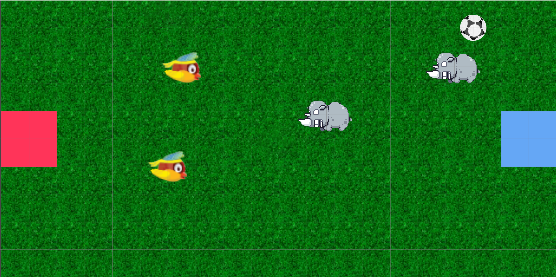
\includegraphics[width=0.6\linewidth]{sprint3/gamestatus.png}
	\caption{The current game status with goals and textures}
	\label{fig:sprint3status}
\end{figure}
\noindent
Additionally, some temporary textures have been added to the game to get rid of the pink playing field and square players.
These new textures can be seen on \autoref{fig:sprint3status}.
